\documentclass{article}
    
    
    \usepackage{graphicx} % Used to insert images
    \usepackage{adjustbox} % Used to constrain images to a maximum size 
    \usepackage{color} % Allow colors to be defined
    \usepackage{enumerate} % Needed for markdown enumerations to work
    \usepackage{geometry} % Used to adjust the document margins
    \usepackage{amsmath} % Equations
    \usepackage{amssymb} % Equations
    \usepackage{eurosym} % defines \euro
    \usepackage[mathletters]{ucs} % Extended unicode (utf-8) support
    \usepackage[utf8x]{inputenc} % Allow utf-8 characters in the tex document
    \usepackage{fancyvrb} % verbatim replacement that allows latex
    \usepackage{grffile} % extends the file name processing of package graphics 
                         % to support a larger range 
    % The hyperref package gives us a pdf with properly built
    % internal navigation ('pdf bookmarks' for the table of contents,
    % internal cross-reference links, web links for URLs, etc.)
    \usepackage{hyperref}
    \usepackage{longtable} % longtable support required by pandoc >1.10
    \usepackage{booktabs}  % table support for pandoc > 1.12.2
    \usepackage{indentfirst}
    \usepackage{floatrow}
    \usepackage{relsize}
    
    \newcommand\perm[2]{{}_{#1}P_{#2}}%
    
    
    \title{Homework 7}
    \author{Roly Vicar\'ia \\ STAT414 Spring 2016}
    
\begin{document}
    
    \maketitle
    
    \textbf{Section 3.1}
    \begin{enumerate}
      \addtocounter{enumi}{1}
      %2
      \item 
	$\mu = \mathlarger{\int}_{-1}^1 x\dfrac{1}{2} dx = \dfrac{x^2}{4} \Big|_{-1}^1 
	  = \dfrac{1}{4} - \dfrac{1}{4} = 0$ \\
	$\sigma^2 = E(X^2) - \mu^2 = \mathlarger{\int}_{-1}^1 x^2 \dfrac{1}{2} dx - 0^2
	  = \dfrac{x^3}{6} \Big|_{-1}^1 = \dfrac{1}{6} + \dfrac{1}{6} = \dfrac{1}{3}$
	
	\begin{figure}[h!]
	  \centering
	  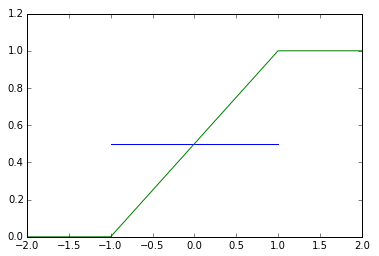
\includegraphics[scale=.5,keepaspectratio=true]{./images/pdf_cdf_U-1-1.png}
	  % pdf_cdf_U-1-1.png: 379x256 pixel, 96dpi, 10.03x6.77 cm, bb=0 0 284 192
	\end{figure}
      
      %3
      \item
	\begin{enumerate}
	 %a
	 \item 
	  $f(x) = \dfrac{1}{10}$ for $0 \le x \le 10$
	 
	 %b
	 \item
	  $P(X \ge 8) = \mathlarger{\int}_8^{10} {\dfrac{1}{10} dx} = \dfrac{x}{10} \Big|_8^{10}
	    = \dfrac{10}{10} - \dfrac{8}{10} = \dfrac{1}{5}$
	 
	 %c
	 \item
	  $P(2 \le X < 8) = \mathlarger{\int}_2^8 {\dfrac{1}{10} dx} = \dfrac{x}{10} \Big|_2^8
	    = \dfrac{8}{10} - \dfrac{2}{10} = \dfrac{6}{10} = \dfrac{3}{5}$
	 
	 %d
	 \item
	  $E(X) = \mathlarger{\int}_0^{10} {x \dfrac{1}{10} dx} = \dfrac{x^2}{20} \Big|_0^{10}
	    = \dfrac{100}{20} - \dfrac{0}{20} = 5$
	 
	 %e
	 \item
	  $Var(X) = E(X^2) - [E(X)]^2 = \mathlarger{\int}_0^{10} {x^2 \dfrac{1}{10} dx} - 5^2
	    = \left[ \dfrac{x^3}{30} \right]_0^{10} - 25 = \dfrac{100}{3} - \dfrac{75}{3} 
	    = \dfrac{25}{3}$
	\end{enumerate}
      
      %4
      \item
	\begin{enumerate}
	 %a
	 \item 
	  $E(X) = \dfrac{5+4}{2} = 4.5$
	  
	 %b
	 \item
	  $Var(X) = \dfrac{(5-4)^2}{12} = \dfrac{1}{12}$
	 
	 %c
	 \item
	  $P(4.2 < X \le 4.7) = \mathlarger{\int}_{4.2}^{4.7} {1 dx} = x \Big|_{4.2}^{4.7}
	    = 4.7 - 4.2 = 0.5$
	\end{enumerate}
      
      %5
      \item
	$F(y) = \mathlarger{\int}_0^y {1 dt} = t \Big|_0^y = y$
	
	\begin{enumerate}
	 %a
	 \item 
	  \begin{align*}
	   G(W) &= P(W \le w) \\
	    &= P(a+(b-a)Y \le w) \\
	    &= P\left(Y \le \dfrac{w-a}{b-a}\right) \\
	    &= F\left(\dfrac{w-a}{b-a}\right) \\
	    &= \dfrac{w-a}{b-a}, a \le w \le b
	  \end{align*}
	 
	 %b
	 \item
	  $U(a,b)$
	\end{enumerate}      
      \addtocounter{enumi}{1}
      
      %7
      \item
	\begin{enumerate}
	 %a
	 \item 
	  \begin{enumerate}
	   %i
	   \item 
	    $1 = \mathlarger{\int}_0^1 {4x^c dx} = 4\left[ \dfrac{x^{c+1}}{c+1} \right]_0^1
	      = 4 \left[ \dfrac{1}{c+1} - 0 \right] = \dfrac{4}{c+1}$ \\
	      
	    Therefore, $c = 3$.
	   
	   %ii
	   \item
	    $F(X) = \mathlarger{\int}_0^x{4t^3 dt} = t^4 \Big|_0^x = x^4$ for $0 \le x \le 1$.
	   
	   %iii
	   \item
	    Pdf (blue) and Cdf (green):
	    \begin{figure}[h!]
	      \centering
	      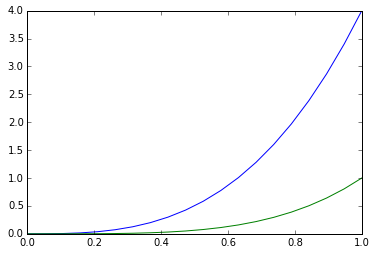
\includegraphics[scale=.6,keepaspectratio=true]{./images/pdf_cdf_7a.png}
	      % pdf_cdf_7a.png: 376x254 pixel, 96dpi, 9.95x6.72 cm, bb=0 0 282 190
	    \end{figure}
	   
	   %iv
	   \item
	    $\mu = \mathlarger{\int}_0^1 {x4x^3 dx} = \dfrac{4x^5}{5} \Big|_0^1 = \dfrac{4}{5}$ \\
	    $\sigma^2 = \mathlarger{\int}_0^1 {x^24x^3 dx} - \left[\dfrac{4}{5}\right]^2
	      = \left[\dfrac{2x^6}{3}\right]_0^1 - \dfrac{16}{25}
	      = \dfrac{2}{3} - \dfrac{16}{25} = \dfrac{2}{75}$
	  \end{enumerate} 
	 
	 \newpage
	 %b
	 \item 
	  \begin{enumerate}
	   %i
	   \item 
	    $1 = \mathlarger{\int}_0^4 {c\sqrt{x} dx} = c \left[\dfrac{2x^{3/2}}{3}\right]_0^4
	      = c \left[\dfrac{16}{3} - 0\right] = \dfrac{16c}{3}$ \\
	      
	    Therefore, $c = \dfrac{3}{16}$.
	   
	   %ii
	   \item
	    $F(X) = \mathlarger{\int}_0^x {\dfrac{3\sqrt{t}}{16} dt} 
	      = \dfrac{3}{16} \left[ \dfrac{2t^{3/2}}{3} \right]_0^x 
	      = \dfrac{3}{16} \left[ \dfrac{2x^{3/2}}{3} \right]
	      = \dfrac{x^{3/2}}{8}$ for $0 \le x \le 4$
	   
	   %iii
	   \item
	    Pdf and Cdf:
	    \begin{figure}[h!]
	      \centering
	      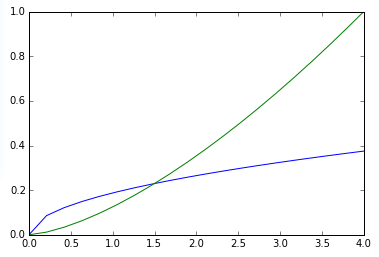
\includegraphics[scale=.6,keepaspectratio=true]{./images/pdf_cdf_7b.png}
	      % pdf_cdf_7b.png: 379x257 pixel, 96dpi, 10.03x6.80 cm, bb=0 0 284 193
	    \end{figure}
	   
	   %iv
	   \item
	    $\mu = \mathlarger{\int}_0^4 {x\dfrac{3}{16}\sqrt{x} dx}
	      = \dfrac{3}{16} \mathlarger{\int}_0^4 {x^{3/2} dx}
	      = \dfrac{3}{16} \left[ \dfrac{2x^{5/2}}{5} \right]_0^4
	      = \dfrac{3}{16} \left(\dfrac{64}{5}\right) = \dfrac{12}{5}$ \\
	    $\sigma^2 = \mathlarger{\int}_0^4 {x^2\dfrac{3}{16}\sqrt{x} dx} - \left[\dfrac{12}{5}\right]^2
	      = \dfrac{3}{16} \left[\dfrac{2x^{7/2}}{7}\right]_0^4 - \dfrac{144}{25}
	      = \dfrac{3}{16}\left(\dfrac{256}{7}\right) - \dfrac{144}{25} = \dfrac{192}{175}$
	  \end{enumerate}
	 
	 %c
	 \item 
	  \begin{enumerate}
	   %i
	   \item 
	    $1 = \mathlarger{\int}_0^1 {\dfrac{c}{x^{3/4}}dx} = c \left[4x^{1/4}\right]_0^1
	      = c \left[ 4(1^{1/4}) - 0 \right] = 4c$ \\
	   
	   Therefore, $c = 1/4$.
	   %ii
	   \item
	    $F(X) = \mathlarger{\int}_0^x {\dfrac{1}{4t^{3/4}}dt} 
	      = \dfrac{1}{4} \mathlarger{\int}_0^x {t^{-3/4}dt} 
	      = \dfrac{1}{4} [4t^{1/4}]_0^x = t^{1/4} \Big|_0^x = x^{1/4}$ for $0 \le x \le 1$
	   
	   %iii
	   \item
	    Pdf and Cdf:
	    \begin{figure}[h!]
	      \centering
	      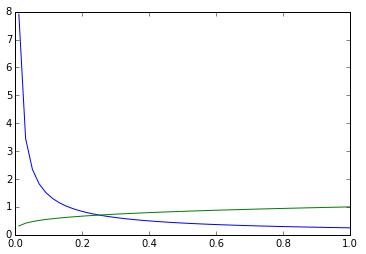
\includegraphics[scale=.6,keepaspectratio=true]{./images/pdf_cdf_7c.png}
	      % pdf_cdf_7c.png: 366x254 pixel, 96dpi, 9.68x6.72 cm, bb=0 0 274 190
	    \end{figure}
	    
	   %iv
	   \item
	    $\mu = \mathlarger{\int}_0^1 {x \dfrac{1}{4x^{3/4}}dx} 
	      = \dfrac{1}{4}\mathlarger{\int}_0^1 {x^{1/4}dx}
	      = \dfrac{1}{4}\left[\dfrac{4x^{5/4}}{5}\right]_0^1
	      = \dfrac{1}{4}\left[\dfrac{4}{5}\right] = \dfrac{1}{5}$ \\
	    
	    $\sigma^2 = \mathlarger{\int}_0^1 {x^2 \dfrac{1}{4x^{3/4}}dx} - \left[\dfrac{1}{5}\right]^2
	      = \dfrac{1}{4}\left[\dfrac{4x^{9/4}}{9}\right]_0^1 - \dfrac{1}{25}
	      = \dfrac{1}{4}\left[\dfrac{4}{9}\right] - \dfrac{1}{25} = \dfrac{16}{225}$
	  \end{enumerate}
	\end{enumerate}	
      \addtocounter{enumi}{1}
      
      %9
      \item
	\begin{enumerate}
	 %a
	 \item 
	  PDF:
	    \begin{figure}[h!]
	      \centering
	      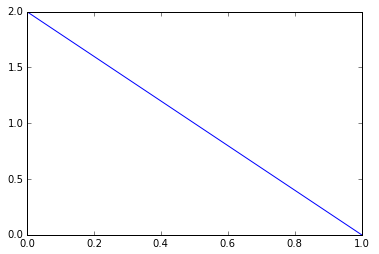
\includegraphics[scale=.5,keepaspectratio=true]{./images/pdf_9a.png}
	      % pdf_9a.png: 379x254 pixel, 96dpi, 10.03x6.72 cm, bb=0 0 284 190
	    \end{figure}
	 
	 %b
	 \item
	  $F(X) = \mathlarger{\int}_0^x {2(1-t)dt} = 2\mathlarger{\int}_0^x {(1-t) dt}
	    = 2\left[t - \dfrac{t^2}{2}\right]_0^x = 2x - x^2$
	  
	  \begin{figure}[h!]
	    \centering
	    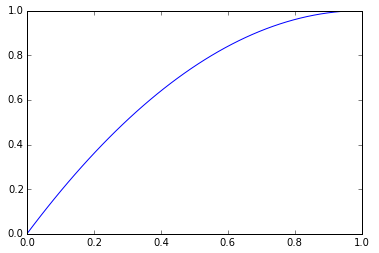
\includegraphics[scale=.5,keepaspectratio=true]{./images/cdf_9b.png}
	    % cdf_9b.png: 379x253 pixel, 96dpi, 10.03x6.69 cm, bb=0 0 284 190
	  \end{figure}

	 
	 %c
	 \item
	  \begin{enumerate}
	   %i
	   \item 
	    $P(0 \le X \le 1/2) = F(1/2)-F(0) = [2(1/2)-(1/2)^2] - 0 = 3/4$
	   
	   %ii
	   \item
	    $P(1/4 \le X \le 3/4) = F(3/4)-F(1/4) = [2(3/4)-(3/4)^2]-[2(1/4)-(1/4)^2] = 1/2$
	   
	   %iii
	   \item
	    $P(X = 3/4) = 0$
	   
	   %iv
	   \item
	    $P(X \ge 3/4) = 1 - P(X \le 3/4) = 1 - F(3/4) = 1 - [2(3/4)-(3/4)^2] = 1/16$
	  \end{enumerate}
	\end{enumerate}
      
      %10
      \item
	\begin{enumerate}
	 %a
	 \item 
	  $\mathlarger{\int}_1^\infty {\dfrac{c}{x^2} dx} 
	    = \mathlarger{\lim}_{b\to\infty}\left[-\dfrac{c}{x}\right]_1^b
	    = \mathlarger{\lim}_{b\to\infty}\left[-\dfrac{c}{b} + c\right] = c$ \\
	    
	 Setting the value above equal to 1, we get that $c=1$.
	 
	 %b
	 \item
	  $\mathlarger{\int}_1^\infty {x \dfrac{1}{x^2} dx}
	    = \mathlarger{\lim}_{b\to\infty}\left[\ln|x|\right]_1^b
	    = \mathlarger{\lim}_{b\to\infty}\left[\ln{b} - \ln{1}\right]
	    = \mathlarger{\lim}_{b\to\infty}\ln{b} = \infty$	  
	\end{enumerate}
      
      %11
      \item
	\begin{enumerate}
	 %a
	 \item
	  $\mathlarger{\int}_1^\infty {\dfrac{d}{y^3}dy}
	    = \mathlarger{\lim}_{b\to\infty}\left[-\dfrac{d}{2y^2}\right]_1^b
	    = \mathlarger{\lim}_{b\to\infty}\left[-\dfrac{d}{2b^2} + \dfrac{d}{2}\right]
	    = \dfrac{d}{2}$ \\
	 
	 Setting the value above equal to 1, we get that $d=2$.
	 
	 %b
	 \item
	  $E(Y) = \mathlarger{\int}_1^\infty {y \dfrac{2}{y^3} dy} 
	    = \mathlarger{\lim}_{b\to\infty} \left[-\dfrac{2}{y}\right]_1^b
	    = \mathlarger{\lim}_{b\to\infty} \left[-\dfrac{2}{b} + 2\right]
	    = 2$
	    
	 %c
	 \item
	  $Var(Y) = \mathlarger{\int}_1^\infty {y^2 \dfrac{2}{y^3} dy}
	    = \mathlarger{\lim}_{b\to\infty} \mathlarger{\int}_1^b {\dfrac{2}{y} dy}
	    = \mathlarger{\lim}_{b\to\infty} \left[2\ln{y}\right]_1^b
	    = \mathlarger{\lim}_{b\to\infty} 2\ln{b} = \infty$
	\end{enumerate}
      \addtocounter{enumi}{2}
      
      \newpage
      %14
      \item
	\begin{enumerate}
	 %a
	 \item 
	  PDF:
	  \begin{figure}[h!]
	    \centering
	    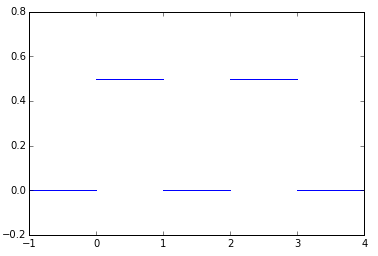
\includegraphics[scale=.5,keepaspectratio=true]{./images/pdf_14a.png}
	    % pdf_14a.png: 378x256 pixel, 96dpi, 10.00x6.77 cm, bb=0 0 283 192
	  \end{figure}
	 
	 %b
	 \item
	  $F(x) =  \begin{cases} 
			0 & x \le 0 \\
			x/2 & 0 < x < 1 \\
			1/2 & 1 \le x \le 2 \\
			(x-1)/2 & 2 < x < 3 \\
			1 & x \ge 3
		    \end{cases}$
	 
	 \begin{figure}[h!]
	    \centering
	    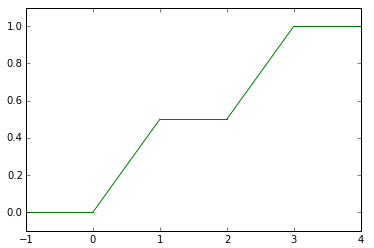
\includegraphics[scale=.5,keepaspectratio=true]{./images/cdf_14b.png}
	    % cdf_14b.png: 374x248 pixel, 96dpi, 9.89x6.56 cm, bb=0 0 280 186
	 \end{figure}
	 
	 %c
	 \item
	  $F(\pi_{0.25}) = \pi_{0.25} / 2 = 0.25$ \\  
	  Therefore, $\pi_{0.25} = 1/2$.
	 
	 %d
	 \item
	  $F(\pi_{0.5}) = 1/2$ \\
	  The cdf evaluates to $1/2$ for $1 \le x \le 2$. So, no, it's not unique.
	 
	 %e
	 \item
	  $F(\pi_{0.75}) = (\pi_{0.75} - 1)/2 = 0.75$ \\ 
	  Therefore, $\pi_{0.75} = 2.5$.
	\end{enumerate}
      
      %15
      \item
	\begin{enumerate}
	 %a
	 \item 
	  \begin{align*}
	    P(X \ge 7) &= 1 - P(X < 7) \\
		      &= 1 - \mathlarger{\int}_0^7 {\dfrac{3x^2}{7^3}e^{-(x/7)^3} dx} \\
		      &= 1 + \left[e^{-(x/7)^3}\right]_0^7 \\
		      &= 1 + \left[e^{-1} - e^{-0}\right] \\
		      &= 1 + \dfrac{1}{e} - 1 \\
		      &= \dfrac{1}{e} \approx 0.3679
	  \end{align*}
	  
	 %b
	 \item
	  \begin{align*}
	   P(X \ge 7 + 3.5 | X \ge 7) &= \dfrac{P((X \ge 10.5) \cap (X \ge 7))}{P(X \ge 7)} \\
		&= \dfrac{P(X \ge 10.5)}{P(X \ge 7)} \\
		&= \dfrac{e^{-(10.5/7)^3}}{1/e} \\
		&= e^{-2.375} \approx 0.0930
	  \end{align*}
	\end{enumerate}
      
      %16
      \item
	$F(x) = \mathlarger{\int}_{-1}^x {\dfrac{t+1}{2} dt} = \dfrac{t^2 + 2t}{4} \Big|_{-1}^x
	  = \dfrac{x^2 + 2x}{4} - \dfrac{(-1)^2 + 2(-1)}{4} = \dfrac{x^2 + 2x}{4} + \dfrac{1}{4}
	  = \left(\dfrac{x+1}{2}\right)^2$
	  
	\begin{enumerate}
	 %a
	 \item 
	  $F(\pi_{0.64}) = \left(\dfrac{\pi_{0.64} + 1}{2}\right)^2 = 0.64$ \\
	  $\pi_{0.64} = 2\sqrt{0.64} - 1 = 2 (\pm0.8) - 1 = -2.6$ or $0.6$
	  
	  Since -2.6 is out of range, $\pi_{0.64} = 0.6$.
	 
	 %b
	 \item
	  $F(\pi_{0.25}) = \left(\dfrac{\pi_{0.25} + 1}{2}\right)^2 = 0.25$ \\
	  $\pi_{0.25} = 2\sqrt{0.25} - 1 = 2 (\pm0.5) - 1 = -2$ or $0$
	  
	  Since -2 is out of range, $\pi_{0.25} = 0$.
	 
	 %c
	 \item
	  $F(\pi_{0.81} = \left(\dfrac{\pi_{0.81} + 1}{2}\right)^2 = 0.81$ \\
	  $\pi_{0.81} = 2\sqrt{0.81} - 1 = 2 (\pm0.9) - 1 = -2.8$ or $0.8$
	  
	  Since -2.8 is out of range, $\pi_{0.81} = 0.8$
	 
	\end{enumerate}

	
    \end{enumerate}

\end{document}